\documentclass[../Carre_nights.tex]{subfiles}

\begin{document}

\section{n0704}
\textbf{\Large{The tale of young Nur and the warrior girl}} \\

\begin{figure}[ht]
\centering
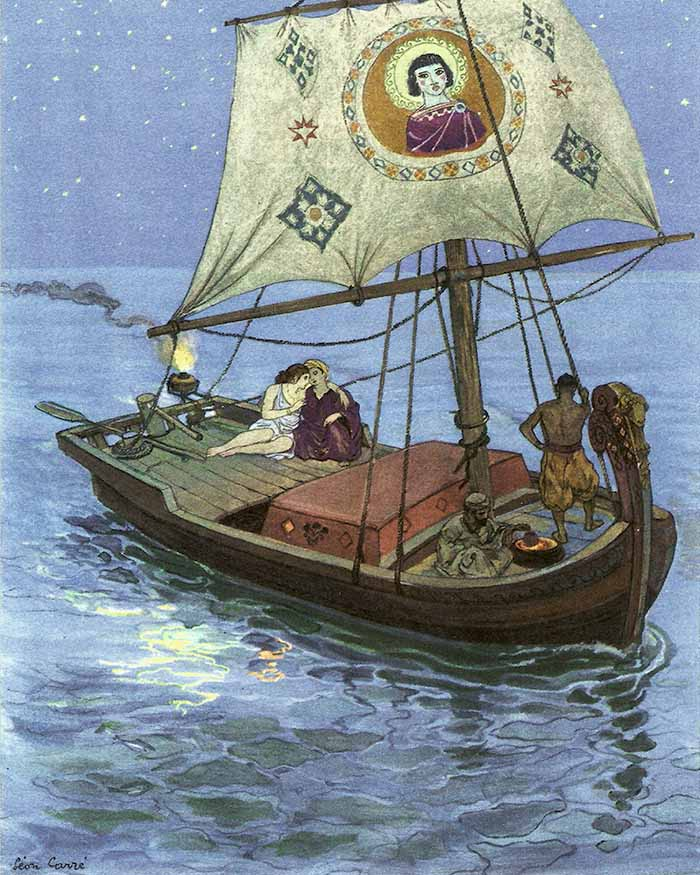
\includegraphics[height=\figsize]{illustrations/volume_6/T06, n0704 - Histoire du jeune Nour avec la franque héroïque.jpg}
\end{figure}

\textit{\\
"...pendant la nuit, elle ne manquait pas d’aller se coucher auprès de son bien-aimé Nour, et de goûter avec lui, dans la fraîcheur marine, sous le ciel nu, toutes les voluptés de l’amour."} \\
—T06, n0704 - Histoire du jeune Nour avec la franque héroïque \\~\\
\textit{"She lay with her beloved each night beneath the naked sky and tasted all delights of him in the sea-fresh air."} \\
—V03, n0704 - The tale of young Nur and the warrior girl

\newpage

\section{n0722}
\textbf{\Large{The strange tale of the mirror of virgins}} \\

\begin{figure}[ht]
\centering
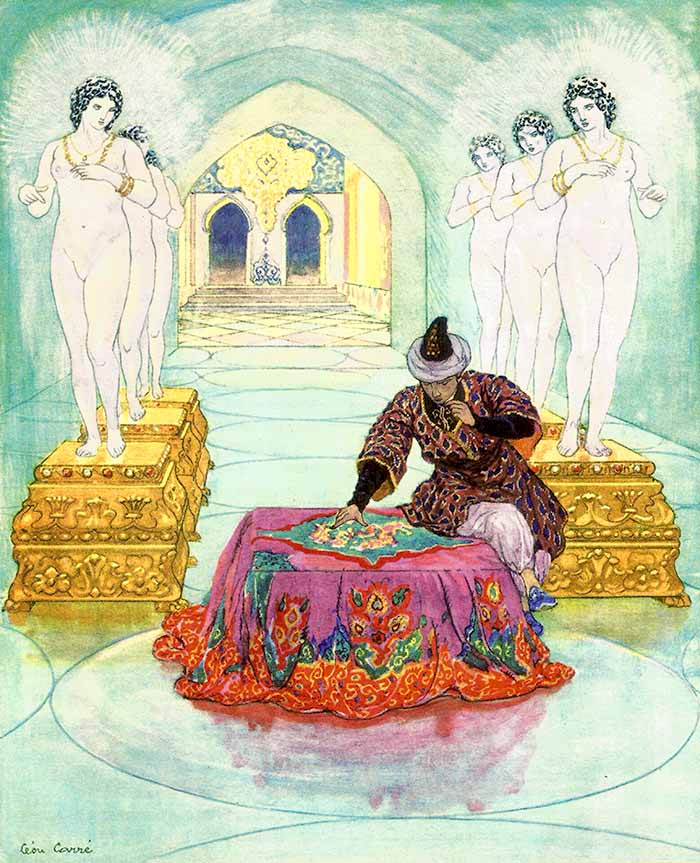
\includegraphics[height=\figsize]{illustrations/volume_6/T06, n0722 - Histoire merveilleuse du miroir des vierges.jpg}
\end{figure}

\textit{\\
"...au milieu de cette salle, sous la voûte, se tenaient debout six adolescentes comme des lunes et brillantes par elles-mêmes d’un tel éclat que la salle en était tout éclairée."} \\
—T06, n0722 - Histoire merveilleuse du miroir des vierges \\~\\
\textit{"...in the middle, under the dome, six girls stood silent on pedestals of solid gold and shone from themselves as if they had been made of moonlight."} \\
—V03, n0722 - The strange tale of the mirror of virgins

\newpage

\section{n0724}
\textbf{\Large{The strange tale of the mirror of virgins}} \\

\begin{figure}[ht]
\centering
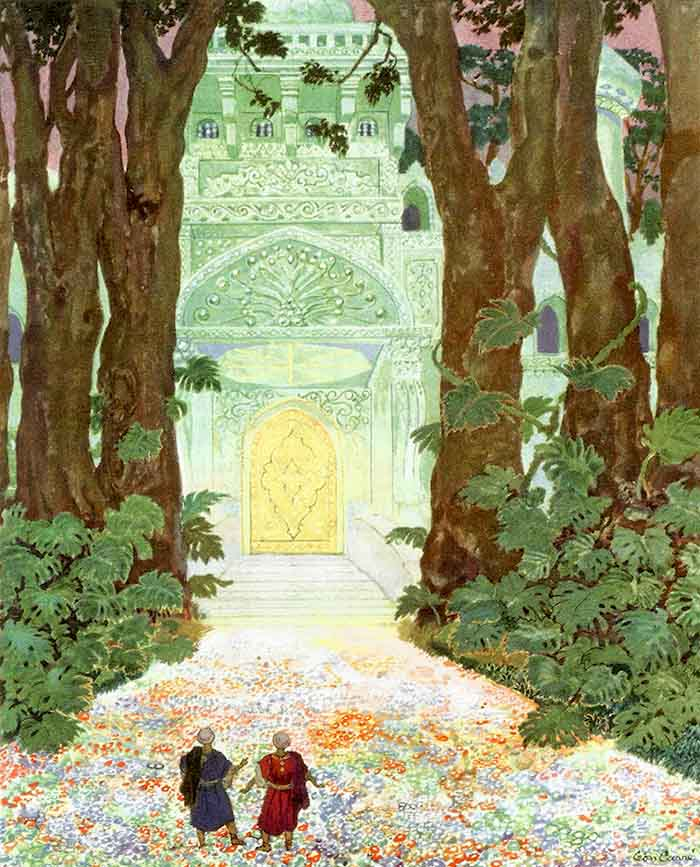
\includegraphics[height=\figsize]{illustrations/volume_6/T06, n0724 - Histoire merveilleuse du miroir des vierges.jpg}
\end{figure}

\textit{\\
"...ils marchèrent ainsi jusqu’à ce qu’ils fussent arrivés devant un palais entièrement construit de pierres d’émeraude, entouré d’un large fossé sur les bords duquel, d’espace en espace, étaient plantés des arbres si hauts qu’ils couvraient de leur ombrage tout le palais."} \\
—T06, n0724 - Histoire merveilleuse du miroir des vierges \\~\\
\textit{"They walked forward until they came to a magnificent palace built up of emeralds, surrounded by a moat, whose outer bank was planted at intervals with trees so tall that they shaded the whole building."} \\
—V03, n0724 - The strange tale of the mirror of virgins

\newpage

\section{n0736}
\textbf{\Large{The tale of Ala al-Din and the wonderful lamp}} \\

\begin{figure}[ht]
\centering
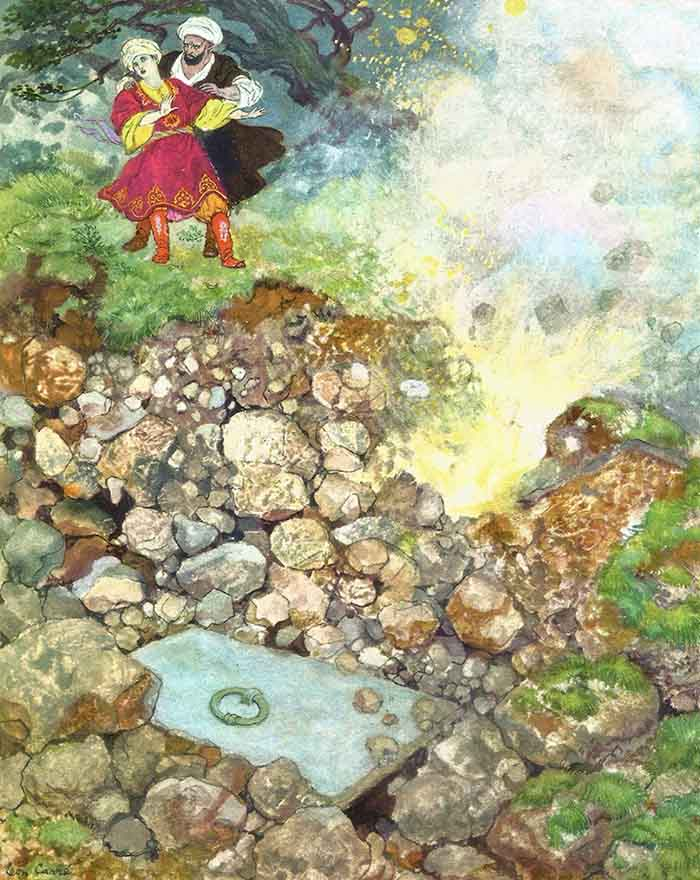
\includegraphics[height=\figsize]{illustrations/volume_6/T06, n0736 - Histoire d'Aladdin et de la lampe magique.jpg}
\end{figure}

\textit{\\
"...une fumée fort épaisse s’éleva qu’il se mit à détourner de côté et d’autre avec ses mains, en marmonnant des formules dans une langue tout à fait inconnue d’Aladdin."} \\
—T06, n0736 - Histoire d'Aladdin et de la lampe magique \\~\\
\textit{"A thick smoke immediately rose, which he waved from side to side with his hand, muttering spells in an unknown tongue."} \\
—V03, n0736 - The tale of Ala al-Din and the wonderful lamp

\newpage

\section{n0745}
\textbf{\Large{The tale of Ala al-Din and the wonderful lamp}} \\

\begin{figure}[ht]
\centering
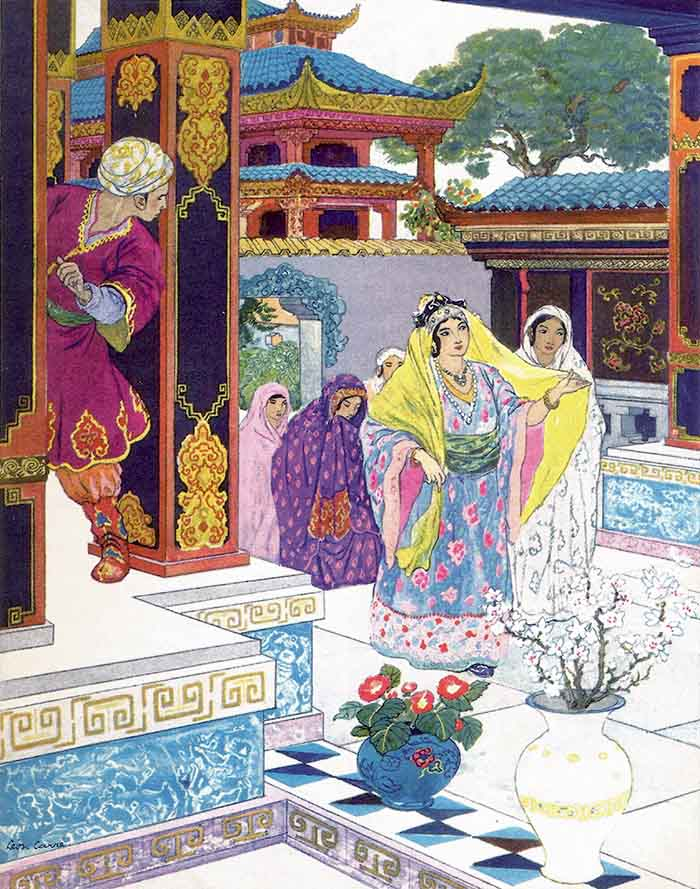
\includegraphics[height=\figsize]{illustrations/volume_6/T06, n0745 - Histoire d'Aladdin et de la lampe magique.jpg}
\end{figure}

\textit{\\
"...il vit arriver le cortège de la princesse, précédé par la foule des eunuques. Et il la vit elle-même au milieu de ses femmes, comme la lune au milieu des étoiles..."} \\
—T06, n0745 - Histoire d'Aladdin et de la lampe magique \\~\\
\textit{"...a crowd of eunuchs appeared, making way for the princess's train. Ala al-Din saw her among her women, a little moon outshining a host of stars..."} \\
—V03, n0745 - The tale of Ala al-Din and the wonderful lamp

\newpage

\section{n0760}
\textbf{\Large{The tale of Ala al-Din and the wonderful lamp}} \\

\begin{figure}[ht]
\centering
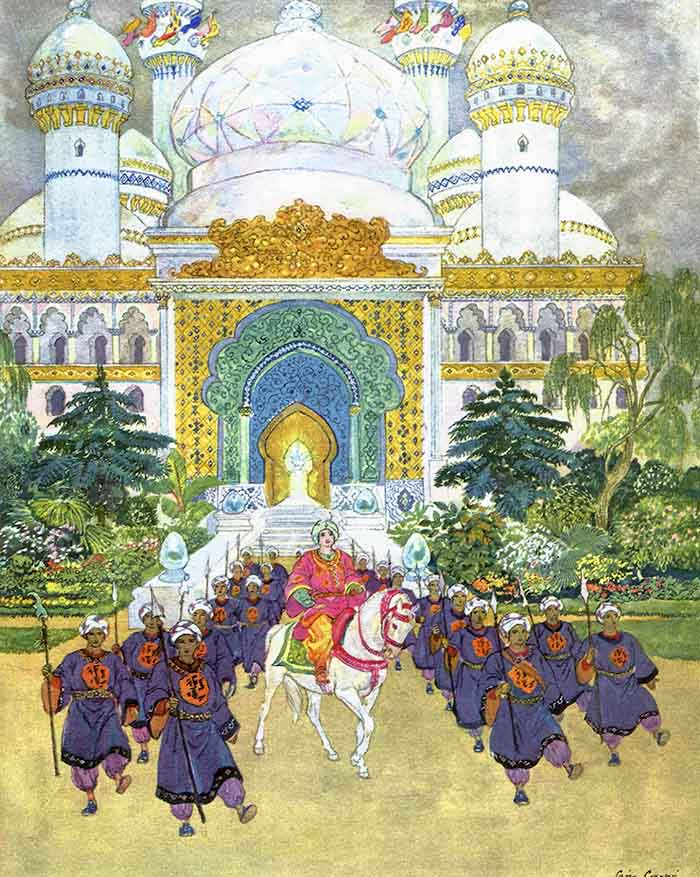
\includegraphics[height=\figsize]{illustrations/volume_6/T06, n0760 - Histoire d'Aladdin et de la lampe magique.jpg}
\end{figure}

\textit{\\
"Prends soin seulement de m’élever, au milieu de ce palais, un grand dôme de cristal construit sur des colonnes d’or massif et d’argent, alternativement..."} \\
—T06, n0760 - Histoire d'Aladdin et de la lampe magique \\~\\
\textit{"...I insist upon one particular: in the middle of the palace you must raise me a vast crystal dome supported by columns of alternate gold and silver..."} \\
—V03, n0760 - The tale of Ala al-Din and the wonderful lamp

\newpage

\section{n0774}
\textbf{\Large{The tale of Ala al-Din and the wonderful lamp}} \\

\begin{figure}[ht]
\centering
\includegraphics[height=\figsize]{illustrations/volume_6/T06, n0774 - Histoire d’Aladdin et de la lampe magique.jpg}
\end{figure}

\textit{\\
"...ils vécurent de la vie bien heureuse, avec la bonne vieille mère d’Aladdin, et avec le sultan, père de Badrou’l-Boudour. Et ils eurent des enfants beaux comme des lunes."} \\
—T06, n0774 - Histoire d’Aladdin et de la lampe magique \\~\\
\textit{"...they lived happily for many years in company with Ala al-Din's mother, that good old woman, and the aged Sultan, who was Badr al-budur's father, and had many children, each as beautiful as the moon."} \\
—V03, n0774 - The tale of Ala al-Din and the wonderful lamp

\newpage

\section{n0774}
\textbf{\Large{The parable of true learning}} \\

\begin{figure}[ht]
\centering
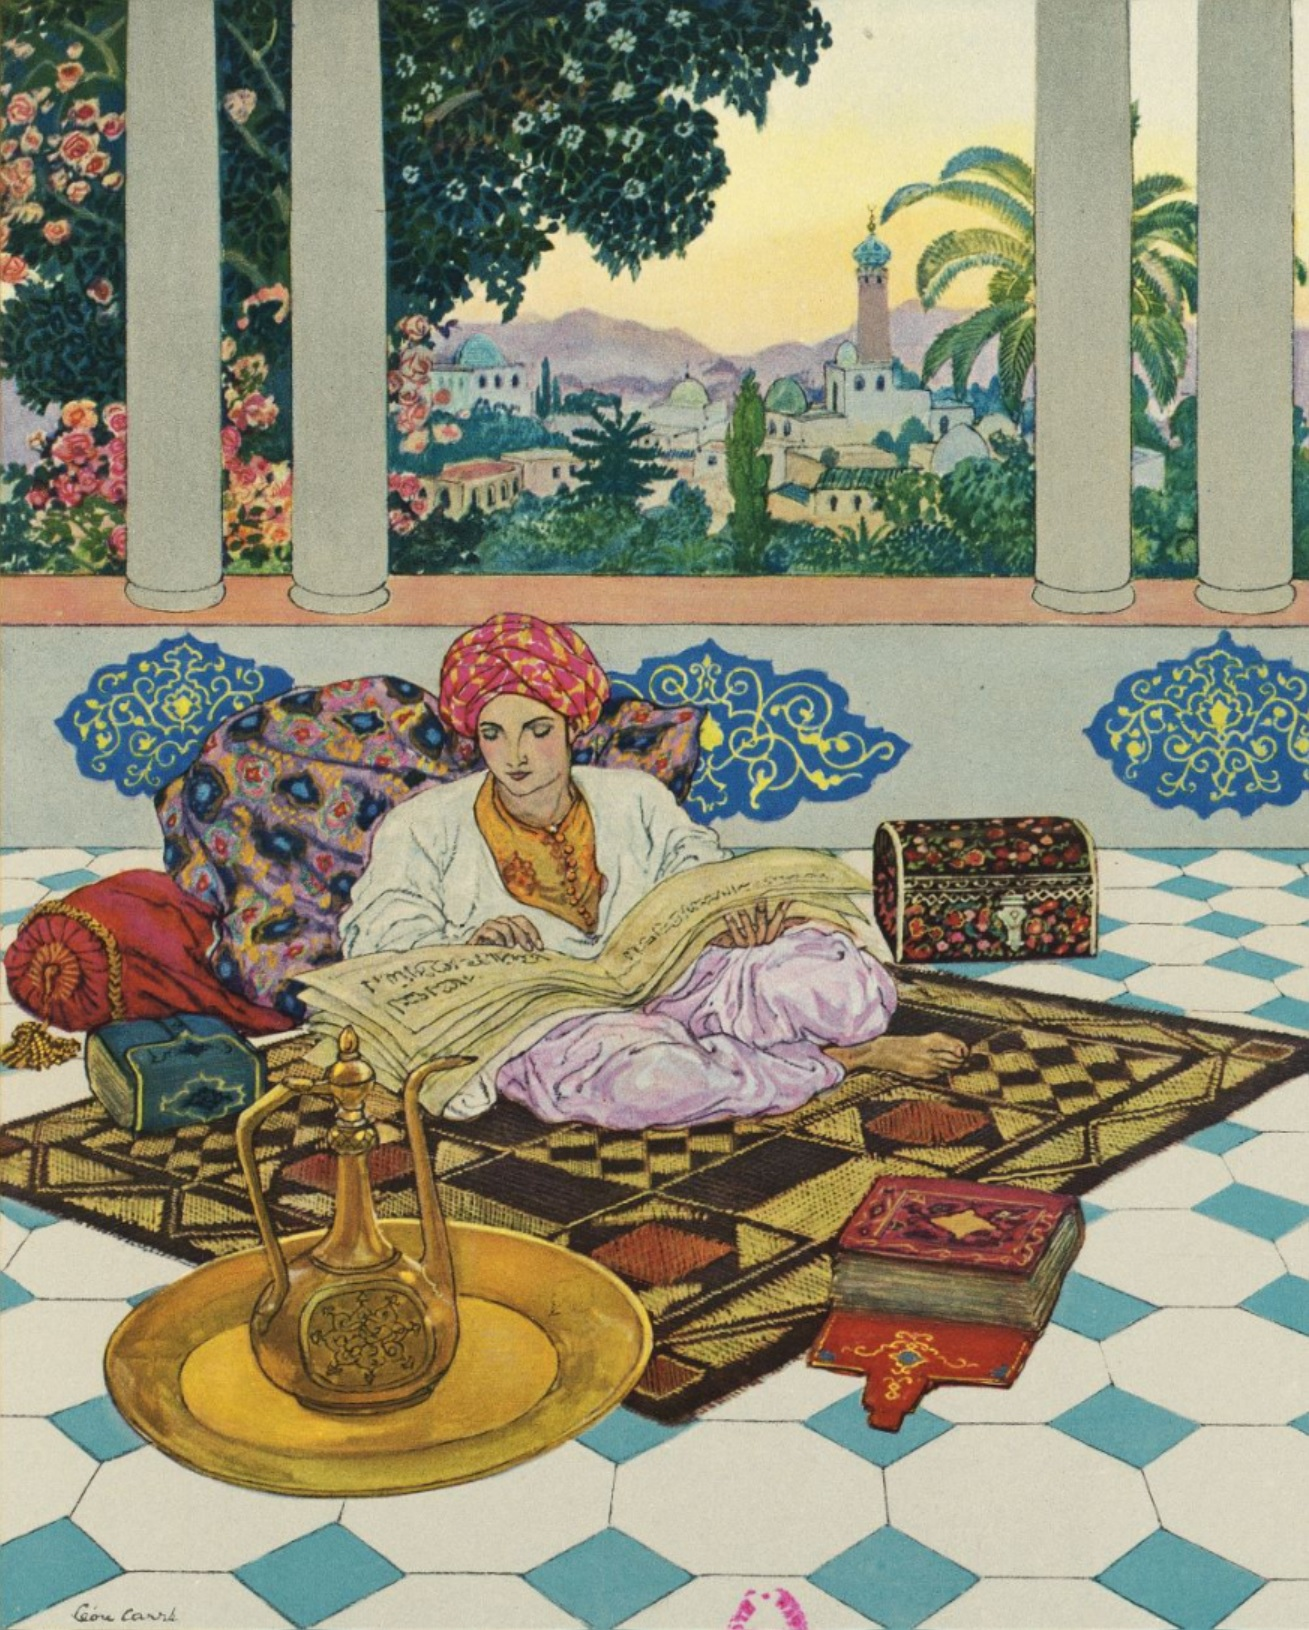
\includegraphics[height=\figsize]{illustrations/volume_6/T06, n0774 - La parabole de la vraie science de la vie.jpg}
\end{figure}

\textit{\\
"...le disciple s’en retourna illuminé dans son pays, au milieu de ses amis ; et il vit clair dans la vie."} \\
—T06, n0774 - La parabole de la vraie science de la vie \\~\\
\textit{"...the young man returned to his own country, as one inspired with light, one who sees clearly."} \\
—V03, n0774 - The parable of true learning

\newpage

\section{n0776}
\textbf{\Large{Farizad of the rose’s smile}} \\

\begin{figure}[ht]
\centering
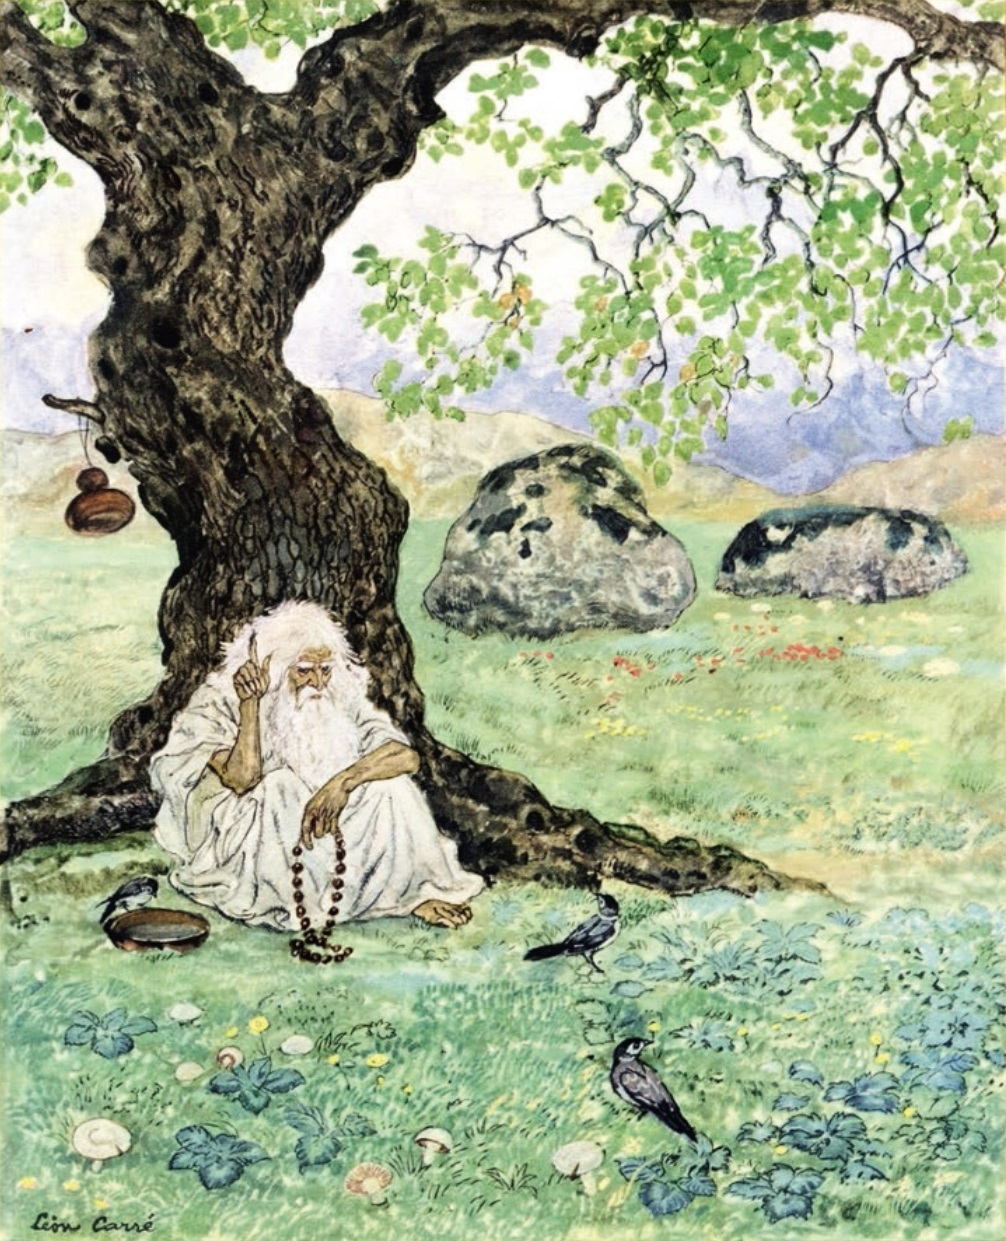
\includegraphics[height=\figsize]{illustrations/volume_6/T06, n0776 - Farizade au sourire de rose.jpg}
\end{figure}

\textit{\\
"...il égrenait de la main gauche un chapelet, tandis qu’il tenait la main droite immobile à la hauteur de son front, avec l’index levé, selon le rite, pour attester l’Unité du Très-Haut."} \\
—T06, n0776 - Farizade au sourire de rose \\~\\
\textit{"With his left hand he told a chaplet of beads, while he held his right immovable at the height of his brow with the index finger raised, to attest the unity of Allah."} \\
—V03, n0776 - Farizad of the rose’s smile

\newpage

\section{n0779}
\textbf{\Large{Farizad of the rose’s smile}} \\

\begin{figure}[ht]
\centering
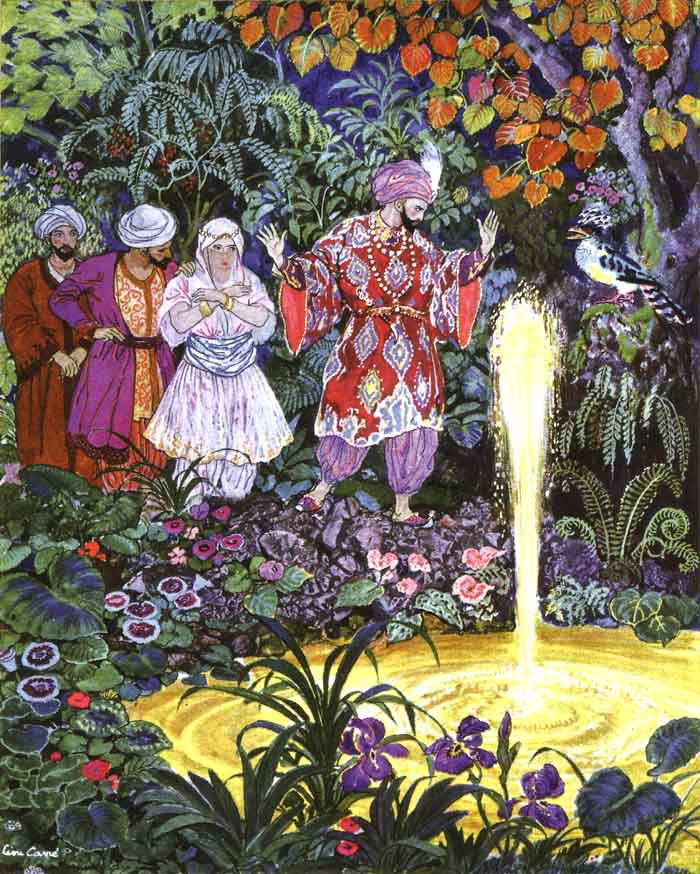
\includegraphics[height=\figsize]{illustrations/volume_6/T06, n0779 - Farizade au sourire de rose.jpg}
\end{figure}

\textit{\\
"...la première chose qui frappa les yeux du sultan Khosrou Schah fut la gerbe d’eau couleur d’or. Et il s’arrêta un moment à la regarder avec admiration..."} \\
—T06, n0779 - Farizade au sourire de rose \\~\\
\textit{"The first marvel which struck the eyes of Khusrau Shah was the spray of Gold Water. He paused for a moment before it..."} \\
—V03, n0779 - Farizad of the rose’s smile

\newpage

\section{n0781}
\textbf{\Large{The tale of Kamar and the expert Halimah}} \\

\begin{figure}[ht]
\centering
\includegraphics[height=\figsize]{illustrations/volume_6/T06, n0781 - Histoire de Kamar et de l’experte Halima.jpg}
\end{figure}

\textit{\\
"...dès qu’ils eurent franchi le seuil de leur maison et fait quelques pas dans la rue, ils se virent entourés par les allants et les venants qui s’arrêtaient sur leur passage, troublés, à l’extrême limite du trouble, par l’adolescent et par sa beauté pleine de damnation pour les âmes."} \\
—T06, n0781 - Histoire de Kamar et de l’experte Halima \\~\\
\textit{"...no sooner had they left the threshold and ventured into the street than they were surrounded by a crowd of passengers, who halted in trouble of spirit, snared by the sweet damnation of Kamar's looks."} \\
—V03, n0781 - The tale of Kamar and the expert Halimah

\newpage

\section{n0792(1)}
\textbf{\Large{The keys of destiny}} \\

\begin{figure}[ht]
\centering
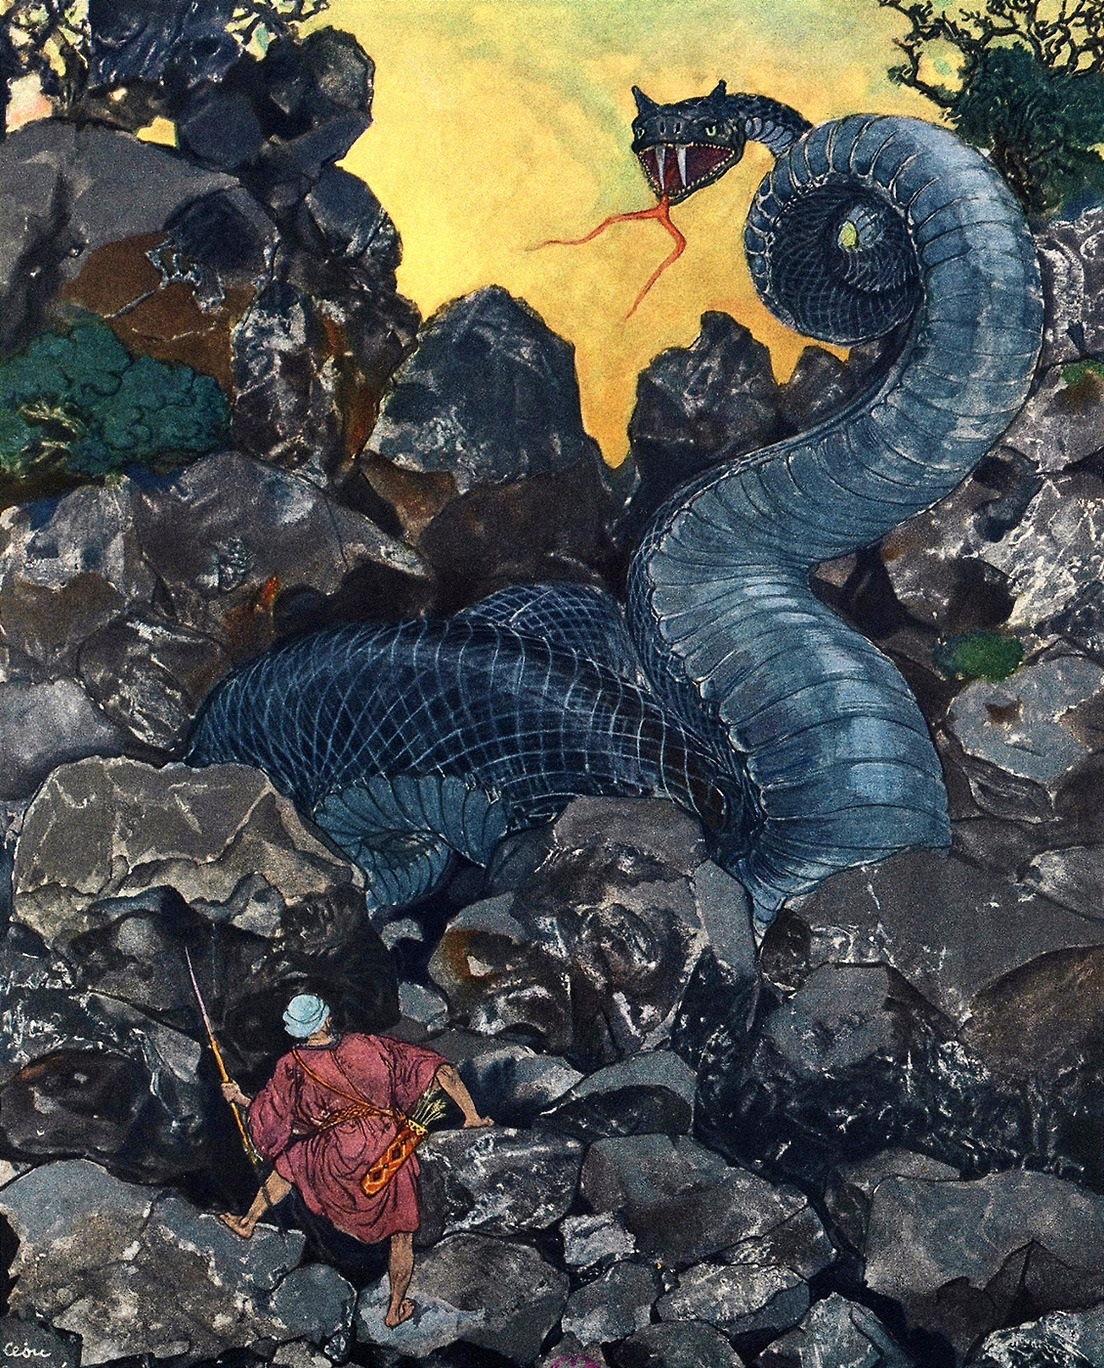
\includegraphics[height=\figsize]{illustrations/volume_6/T06, n0792(1) - Les clefs du destin.jpg}
\end{figure}

\textit{\\
"...je fondis en larmes, et reconnus en mon âme que je n’avais rien à refuser à l’homme qui avait sauvé ma maison et ceux de ma maison. Et je pris en tremblant l’arc et la flèche, et je me dirigeai vers les rochers noirs où je voyais rouler les reptiles terrifiants. Et je ne fus pas longtemps sans découvrir celui que je cherchais..."} \\
—T06, n0792(1) - Les clefs du destin \\~\\
\textit{"...I burst into tears and, taking the bow and arrow in my trembling hands, walked towards the black rocks, in and out of which serpents of the same colour writhed in terrifying knots. It was not long before I found my prey..."} \\
—V03, n0792(1) - The keys of destiny

\newpage

\section{n0792(2)}
\textbf{\Large{The keys of destiny}} \\

\begin{figure}[ht]
\centering
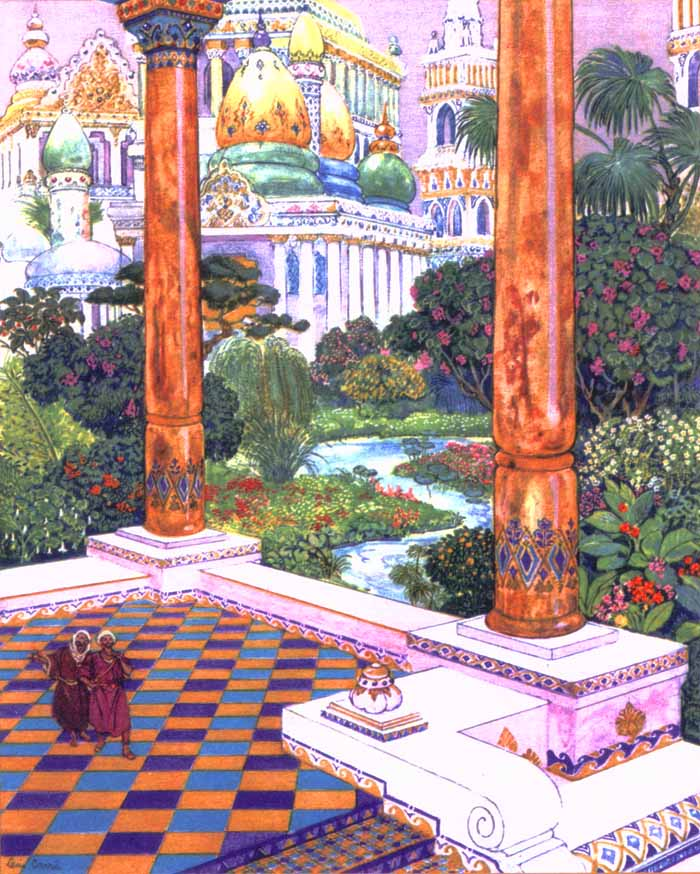
\includegraphics[height=\figsize]{illustrations/volume_6/T06, n0792(2) - Les clefs du destin.jpg}
\end{figure}

\textit{\\
"...nous traversâmes des rues bordées de palais à colonnades, d’albâtre et des jardins où l’air respiré était de lait et les ruisseaux d’eaux embaumées."} \\
—T06, n0792(2) - Les clefs du destin \\~\\
\textit{"We passed through streets bordered by palaces with colonnades of alabaster, and by gardens where the air was milk and the streams ran flower-water."} \\
—V03, n0792(2) - The keys of destiny

\newpage

\section{n0811}
\textbf{\Large{The tale of princess Nur al-Nihar}} \\

\begin{figure}[ht]
\centering
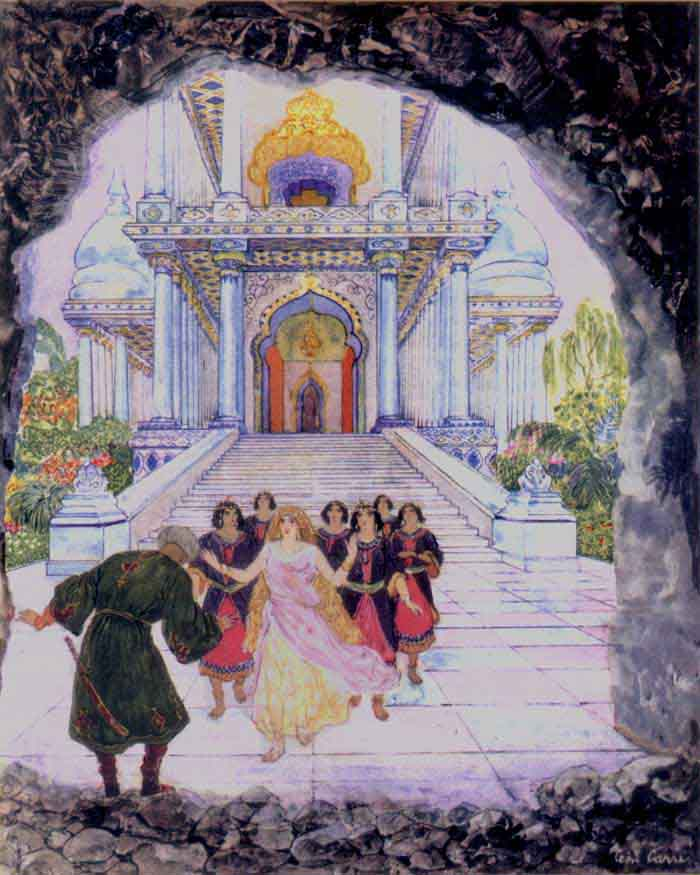
\includegraphics[height=\figsize]{illustrations/volume_6/T06, n0811 - Histoire de la princesse Nourennahar.jpg}
\end{figure}

\textit{\\
"...avant qu’il eût le temps d’admirer l’architecture de ce palais, une dame en sortit qui s’avança vers lui, entourée d’une troupe d’autres dames, et dont, à n’en pas douter, elle était la maîtresse, à en juger seulement par sa beauté miraculeuse et son port majestueux."} \\
—T06, n0811 - Histoire de la princesse Nourennahar \\~\\
\textit{"As he looked, a lady came out of the palace followed by a group of damsels, and he was sure, from her queenly carriage and perfect beauty, that she was the mistress and those the slaves."} \\
—V03, n0811 - The tale of princess Nur al-Nihar

\end{document}